

\chapter{Unions}\label{chap:unions}

\section{Introduction}

This chapter will consist of a brief discussion of how multi-structures are ``summed". The sum is similar to computing the union of sets (more specifically multi-sets), but with major differences as will soon become apparent.

A ``union" between two multi-structures of the same ``type" is the result of simply ``combining" the multi-structures in a straightforwards manner. The addition symbol ``\(+\)" denotes the union. The union of two sets typically counts the elements that are common to both sets only once, but here {\bf the weights of structures that are common to both multi-structures are added together}. 

{\bf Only multi-structures with the same type can be summed. The sum/union of multi-structures of different types will not be considered.} 


\section{point-point unions}

\vspace{5mm}

\begin{tabular}{cc}
\parbox{0.5\textwidth}{
The union of multi-points \(\rho_1\) and \(\rho_2\) is the set of all weighted points from both multi-points. If the same points appear then their weights are added. If any resultant weight is \(0\), then the corresponding point disappears.  

An example of such a multi-point union is depicted on the right. Illustrated are examples of points stacking up to form points of greater weight, and points canceling out, partially as well as completely. 
} & \parbox{0.5\textwidth}{
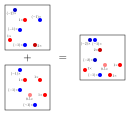
\includegraphics[width = 0.5\textwidth]{Unions/multipoint_unions}
}
\end{tabular}

Lastly, given a multi-point \(\rho\) and a positive integer \(n\), then
\[n \cdot \rho = \underbrace{\rho + \rho + ... + \rho}_n\]
so ``multiplying" a multi-point by \(n\) is to multiply the weight of each point by \(n\). More generally, to multiply a multi-point by any real number \(k\) is to multiply the weight of each point by \(k\). ``Multiplication" by \(k\) is denoted by:
\[k \cdot \rho \quad\quad\text{or}\quad\quad k\rho \quad\quad\text{or}\quad\quad \rho \cdot k \quad\quad\text{or}\quad\quad \rho k\]


\section{path-path unions}

\vspace{5mm}

\begin{tabular}{cc}
\parbox{0.5\textwidth}{
The union of multi-paths \(\mathbf{J}_1\) and \(\mathbf{J}_2\) is the set of all weighted oriented paths from both multi-paths. An example of such a union is depicted on the right. Illustrated are examples of paths with identical orientation stacking to form paths with a greater weight, and paths with opposite orientation canceling out.
} & \parbox{0.5\textwidth}{
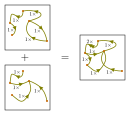
\includegraphics[width = 0.5\textwidth]{Unions/multipath_unions}
}
\end{tabular}

Lastly, given a multi-path \(\mathbf{J}\) and a positive integer \(n\), then
\[n \cdot \mathbf{J} = \underbrace{\mathbf{J} + \mathbf{J} + ... + \mathbf{J}}_n\]
so ``multiplying" a multi-path by \(n\) is to multiply the weight of each path by \(n\). More generally, to multiply a multi-path by any real number \(k\) is to multiply the weight of each path by \(k\), reversing the orientation of paths with negative weight. ``Multiplication" by \(k\) is denoted by:
\[k \cdot \mathbf{J} \quad\quad\text{or}\quad\quad k\mathbf{J} \quad\quad\text{or}\quad\quad \mathbf{J} \cdot k \quad\quad\text{or}\quad\quad \mathbf{J} k\]


\section{surface-surface unions}

\vspace{5mm}

\begin{tabular}{cc}
\parbox{0.5\textwidth}{
The union of multi-surfaces \(\mathbf{F}_1\) and \(\mathbf{F}_2\) is the set of all weighted oriented surfaces from both multi-surfaces. An example of such a union is depicted on the right (using 2D cross-sections). Illustrated are examples of surfaces with identical orientation stacking to form surfaces with a greater weight, and surfaces with opposite orientation canceling out, partially as well as completely.
} & \parbox{0.5\textwidth}{
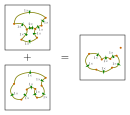
\includegraphics[width = 0.5\textwidth]{Unions/multisurface_unions}
}
\end{tabular}

Lastly, given a multi-surface \(\mathbf{F}\) and a positive integer \(n\), then
\[n \cdot \mathbf{F} = \underbrace{\mathbf{F} + \mathbf{F} + ... + \mathbf{F}}_n\]
so ``multiplying" a multi-surface by \(n\) is to multiply the weight of each surface by \(n\). More generally, to multiply a multi-surface by any real number \(k\) is to multiply the weight of each surface by \(k\), reversing the orientation of surfaces with negative weight. ``Multiplication" by \(k\) is denoted by:
\[k \cdot \mathbf{F} \quad\quad\text{or}\quad\quad k\mathbf{F} \quad\quad\text{or}\quad\quad \mathbf{F} \cdot k \quad\quad\text{or}\quad\quad \mathbf{F} k\]



\section{volume-volume unions}

\vspace{5mm}

\begin{tabular}{cc}
\parbox{0.5\textwidth}{
The union of multi-volumes \(U_1\) and \(U_2\) is the set of all weighted volumes from both multi-volumes. An example of such a union is depicted on the right (using 2D cross-sections). Illustrated are examples of volumes partially canceling each other out. Note that for a specific point \(\mathbf{q}\), that the net number of volumes that contain \(\mathbf{q}\) in the union \(U_1 + U_2\) will always be the sum of the net number of volumes that contain \(\mathbf{q}\) in each of \(U_1\) and \(U_2\): 
\[(U_1 + U_2)(\mathbf{q}) = U_1(\mathbf{q}) + U_2(\mathbf{q})\]
} & \parbox{0.5\textwidth}{
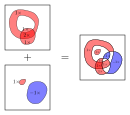
\includegraphics[width = 0.5\textwidth]{Unions/multivolume_unions}
}
\end{tabular}

Lastly, given a multi-volume \(U\) and a positive integer \(n\), then
\[n \cdot U = \underbrace{U + U + ... + U}_n\]
so ``multiplying" a multi-volume by \(n\) is to multiply the weight of each volume by \(n\). More generally, to multiply a multi-volume by any real number \(k\) is to multiply the weight of each volume by \(k\). ``Multiplication" by \(k\) is denoted by:
\[k \cdot U \quad\quad\text{or}\quad\quad k U \quad\quad\text{or}\quad\quad U \cdot k \quad\quad\text{or}\quad\quad U k\]




\section{Summary}

This chapter was a brief formalization of the union of two multi-structures with the same type. The union of multi-structures with different types is not allowed.


